\section{CAG Register File Generator}
To resolve the problems connected with commercial tools for RFs the Computer Architecture Group (CAG) of the Heidelberg University is developing its own tool called Register File Generator (RFG). It is an open source project and publicly available at \emph{github.com/unihd-cag/odfi-rfg}.

\subsection{RFG Terminology}

The RFG uses two interfaces to access the generated RF (fig.~\ref{fig::rfg_view}). On one side a bus, which enables access to the RF from outside the hardware and is called software view. Its signals shared between the registers of the RF and a specific CSR is accessed via its address. Thereby different read or write commands targeting the RF can only be executed sequentially.\\
On the contrary the logic of the hardware is directly connected to each of its corresponding registers (except memory based registers as descriped in section~\ref{section::ramblocks}). Therefore the interface of the hardware view does not represent an uniform set of signals, but rather an aggregation of point-to-point connections.

\begin{figure}[h]
 \centering
 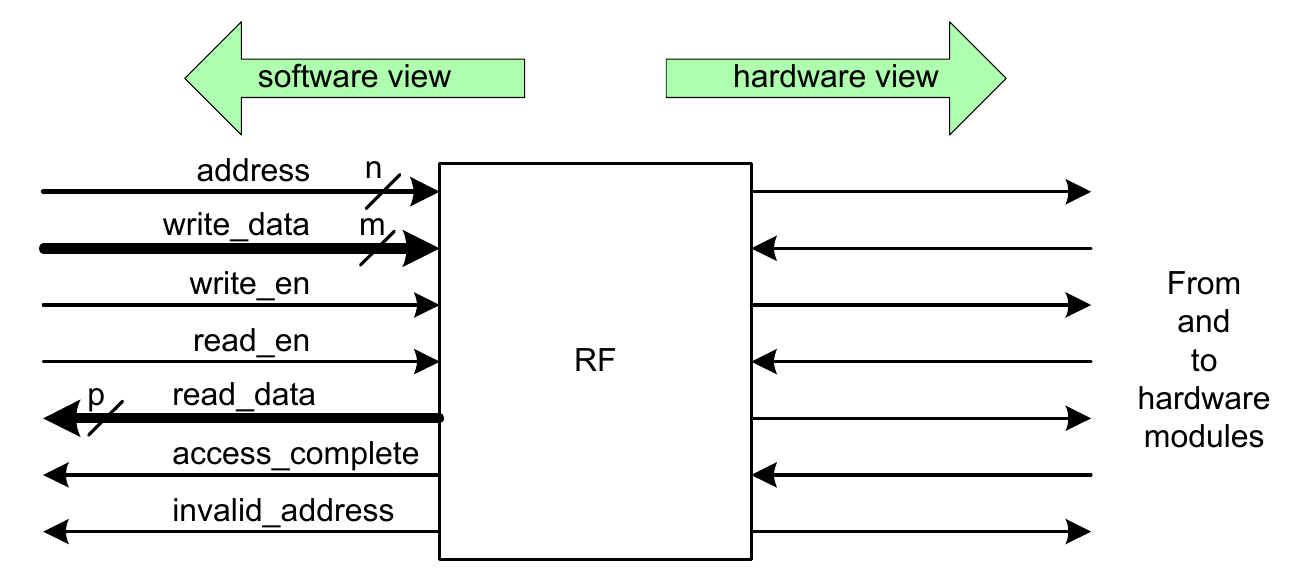
\includegraphics[width=252pt]{images/rf_view.png}
 \caption{RFG Terminology \cite{leber_diss}}
\label{fig::rfg_view}
\end{figure}

\begin{figure}[h]
 \centering
 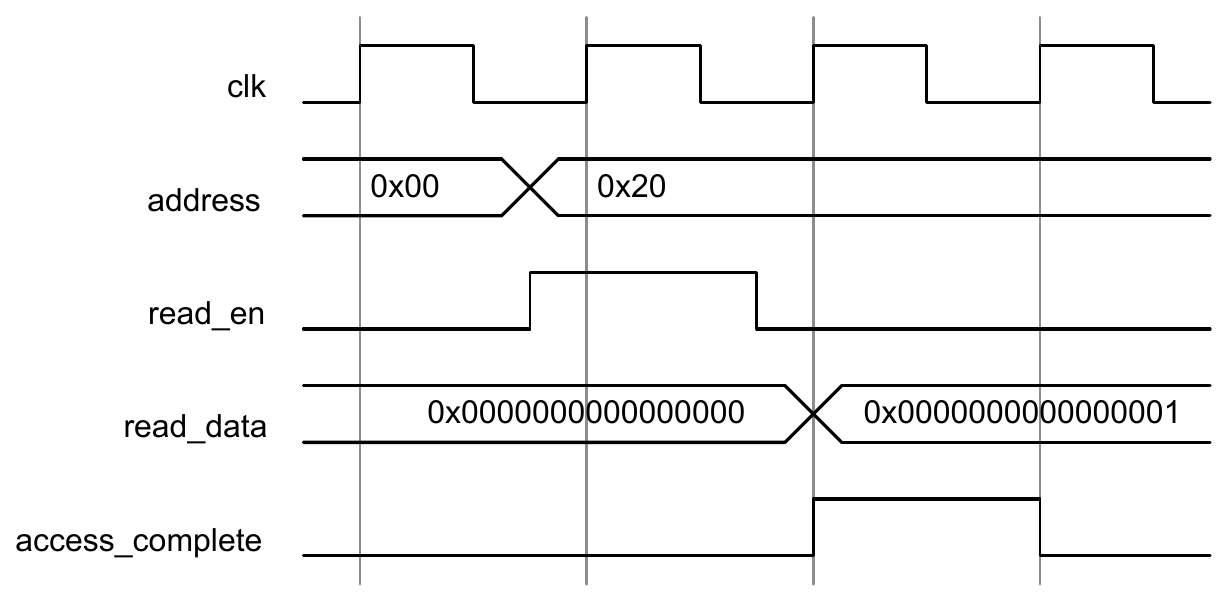
\includegraphics[width=252pt]{images/sw_read_timing.png}
 \caption{Timing Diagram of a SW Read Access \cite{leber_diss}}
\label{fig::sw_read}
\end{figure}

\begin{figure}[h]
 \centering
 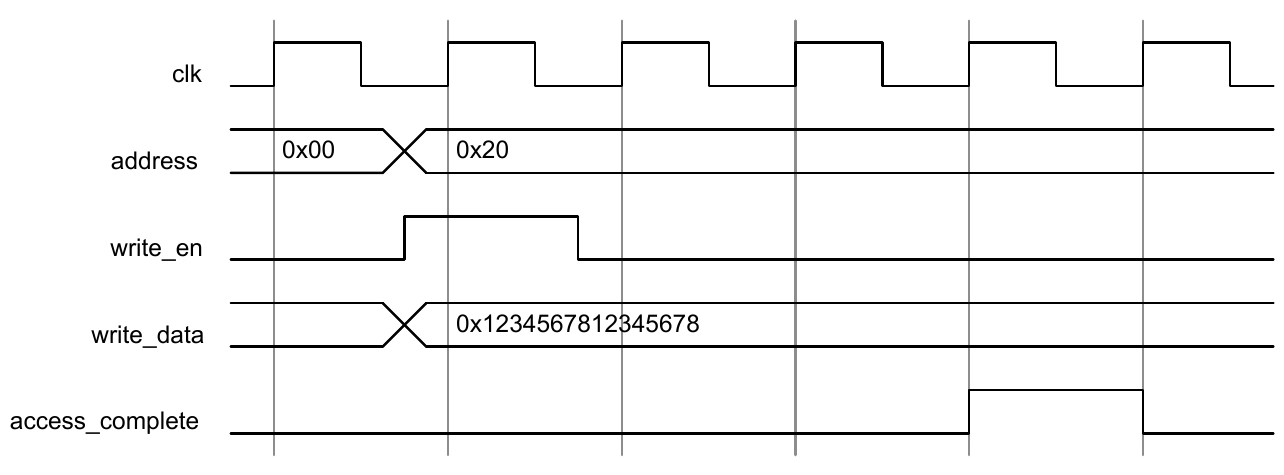
\includegraphics[width=252pt]{images/sw_write_timing.png}
 \caption{Timing Diagram of a SW Read Access \cite{leber_diss}}
\label{fig::sw_write}
\end{figure}

An example of a RF description for the RFG is given in listing~\ref{lst::example_rf}.

\lstset{language={}, numbers=none, escapechar=|}
\begin{lstlisting}[frame=single,
caption={Example RF description},
basicstyle=\small\ttfamily,
label={lst::example_rf}]
registerFile rf_top {

  register reg0 {
    field field0 {
      width 32
      software {
        rw
      }
      hardware {
        rw
        clear
      }
    }
    reserved 32
  }
	
  ramBlock ram0 {
    width 64
    depth 32
    software rw
    hardware rw
  }
	
  external rf_inner.rf example
}
\end{lstlisting}
\subsection{Register Files}
A RF is the top module containing all other components like registers and ramblocks. It is declared using \lstinline$registerFile$ followed by its name.
Furthermore hierarchical RFs are available, which split the RF in multipe sub-RFs. On the one hand this can resolve timing problems in large designs (see section~\ref{rf_generation}), on the other hand the RF obtains a clear structure and is therefore better to maintain than a non-hierarchical one.\\
A hierarchical RF is created by using the \lstinline$external$ statement followed by the filename of the included RF and the name of the RF. Each RF respectively sub-RF is declared in an individual file using the filename extention \lstinline$.rf$.
\subsection{Registers}
CSRs are declared inside of an RF using the \lstinline$register$ statement followed by an unique name in the scope of the enclosing RF. The width of the registers is declared globally and has the default value of 64 bit. Each register can contain multiple fields with variable width. Thereby, unused sections can be marked with the \lstinline$reserved$ statement. Furthermore read and write permissions can be assigned to each field for both software and hardware view.\\
In addition to the basic CSRs, more specialized registers can be created with this generator. This is achieved by assigning flags to the fields of the register in the RF description called attributes. For example, a counter can be added to the RF by using the corresponding attribute (see \cite{rfg_spec} for a list of available attributes).
\subsection{Ramblocks}\label{section::ramblocks}
The RFG also supports memory type registers in static random-access memories (SRAMs) called ramblocks. These are used when the same kind of register is required multiple times with consecutive addresses. It is important to mention, that in this case the hardware is not directly connected to the fields. Instead the logic can only use an SRAM interface to read or write an entire entry of the memory, which is similar to accessing a complete register.\\
Analogous to the fields of registers, read and write permissions for software and hardware view can be specified for ramblocks. Additionally each ramblock can either be internal (default value) or external. Internal ones are instantiated within the RF, whereas an external ramblock only includes an SRAM interface inside of the RF and the developer has to connect it.
